
\documentclass[10pt]{article}
%	options include 12pt or 11pt or 10pt
%	classes include article, report, book, letter, thesis

\usepackage[a4paper,bindingoffset=0.2in,%
            left=1in,right=1in,top=0.2in,bottom=0.3in,%
            footskip=.15in]{geometry}
            
\usepackage[T1]{fontenc}
\usepackage[polish]{babel}
\usepackage[utf8]{inputenc}
\usepackage{lmodern}
\selectlanguage{polish}
\usepackage{blindtext}
\usepackage{pgfplots}
\usepackage{graphicx}

\title{Algorytmy numeryczne}
\author{Zadanie 2 \\ Aleksander Kosma\\grupa 1 tester-programista}
\date{8 Listopad 2017}

\begin{document}
\maketitle 

\section{Dodawanie i Mnożenie}
// czy jezykz duzej czy malej
Opracowanie prezentuje obliczenia na macierzach, przy użyciu języka Java i wsparciu Eigena 
wykorzystanego w C++.
Pierwsza część opisuje czas działania i błędy operacji dodawania i mnożenia.
Obliczenia wygenerowane w Javie porównywane były z wynikami wygenerowanymi z Eigena.
Testy zostały przeprowadzone na 3 wzorach:
$$A * X$$
$$(A+B+C)*X$$
$$A*B*C$$
Gdzie litery A,B,C to macierze, X to wektor.

Testy zostały przeprowadzone na 3 typach zmiennych. Double, Float i na własnym typie, który przechowuje
liczbę w postaci ułamka. Typ ten ma bezstratną precyzję.


Wykresy obliczone dla Double:\\

Pierwszy wykres prezentuje czas potrzebny do obliczenia podanego wzoru. Pod koniec widać przewagę własnych obliczeń nad Eigen.
\begin{center}
 \makebox[\textwidth]{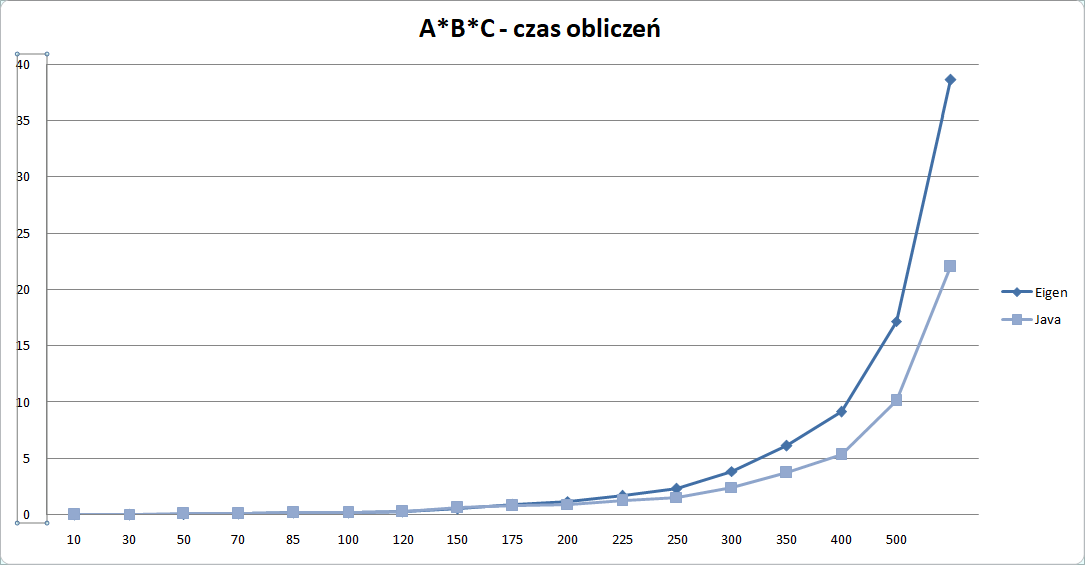
\includegraphics[width=0.7\paperwidth]{ABCCzas.png}}
\end{center}

Drugi wykres prezentuje te same dane, tylko w kontekście precyzji. Widać ze wraz ze wzrostem wielkości macierzy, błędy przybierają na wartości.
\begin{center}
 \makebox[\textwidth]{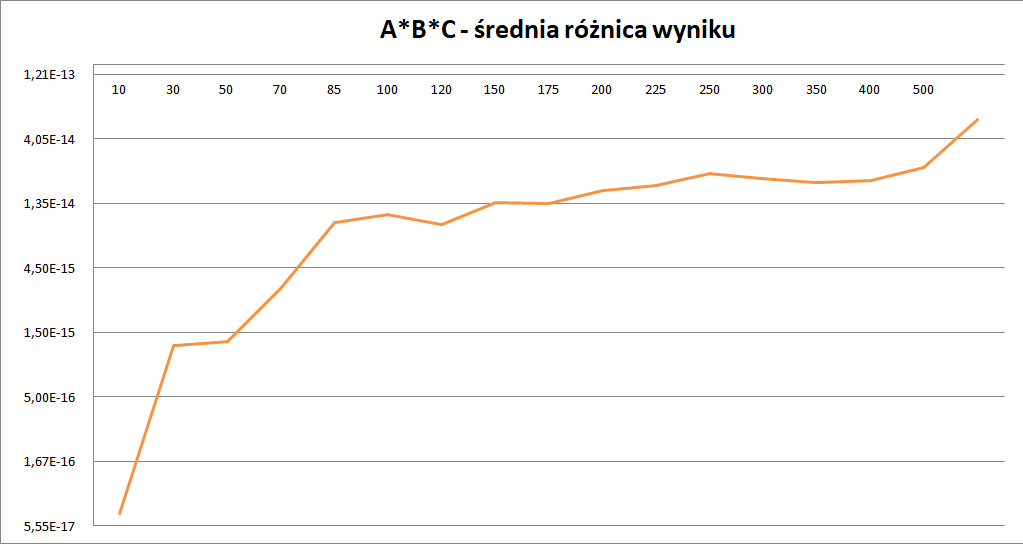
\includegraphics[width=0.7\paperwidth]{ABCRoznica.png}}
\end{center}

Trzeci wykres prezentuje dla innego wzoru czas obliczeń. W pewnym momencie obliczenia Javy stają się szybsze
i tendencja ta się utrzymuje.
\begin{center}
 \makebox[\textwidth]{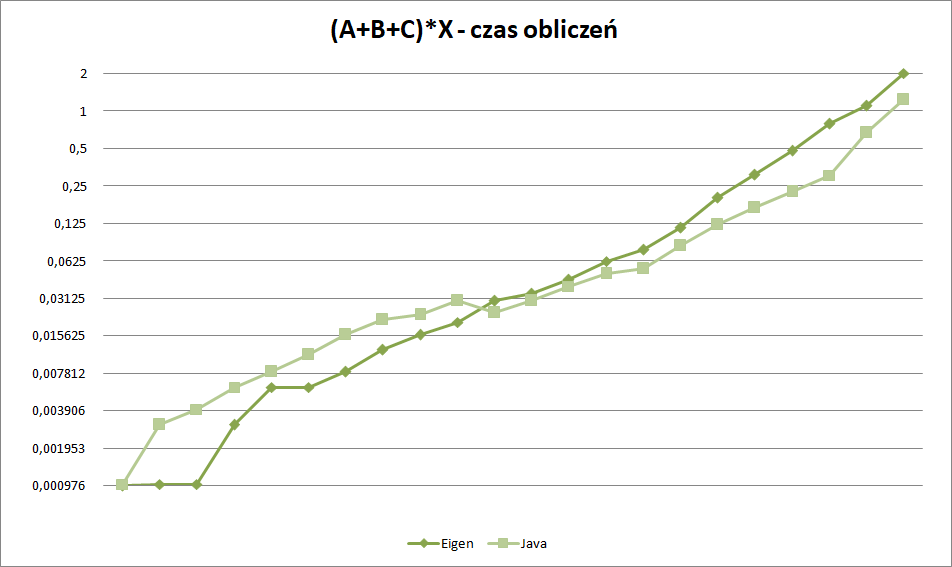
\includegraphics[width=0.7\paperwidth]{ABCXCzas.png}}
\end{center}

Czwarty wykres prezentuje podobne wnioski jak w przypadku pierwszego. Tym większa macierz tym większy błąd ostateczny. 
\begin{center}
 \makebox[\textwidth]{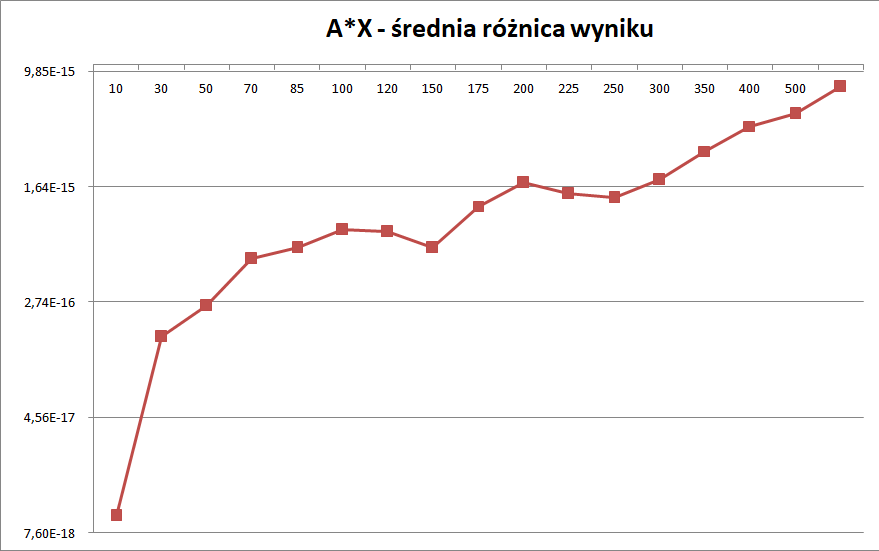
\includegraphics[width=0.7\paperwidth]{AXRoznica.png}}
\end{center}

Obliczenia na Float wykazywały podobną tendencje, tyle że w mniejszej skali i wolniejszym tempie, więc pominę prezentacje dla tej zmiennoprzecinkowej.
W przypadku własnej precyzji, w zakresie porównania do Double obliczonego przez Eigen wyniki pokrywały się idealnie. Główna różnica to dłuższy czas oczekiwania na wynik.

\begin{center}
 \makebox[\textwidth]{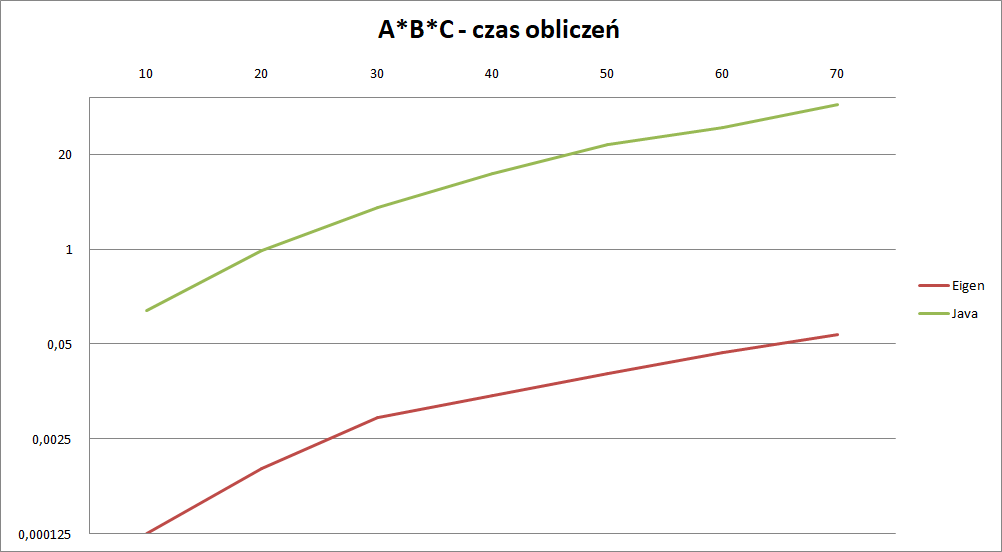
\includegraphics[width=0.7\paperwidth]{ABCCzasMy.png}}
\end{center}



\section{Rozwiązywanie układów równań liniowych}
Druga część opisuje rozwiązywanie układu równań liniowych macierzy A i wektora B.
W Javie wykorzystane zostały 3 wersje metody eliminacji Gaussa:
-bez wyboru elementu podstawowego
-z częściowym wyborem elementu podstawowego
-z pełnym wyborem elementu podstawowego
Odnośnikiem jako poprawny wynik były wektory obliczone przez Eigen. Eigen ma możliwość oblicznia układu poprzez częściowy wybór, albo pełny elementu podstawowego.




\end{document}